\documentclass[final,10pt]{beamer}
\usepackage{upgreek}
\usepackage{multicol}
\usepackage{multimedia}
%options=light OR dark
\usetheme[dark]{agwagnerpresentation}

\setbeamertemplate{headline}{}

\graphicspath{{images-postdoc-tex/}}

%title of the poster
% \title[Application for the post of \textit{postdoctoral fellow in microscopy}]{\small{Application for the post of}\\\Large{\textit{postdoctoral fellow in microscopy}}}
\title[Load Response of the Flagellar Beat]{\Large{Load Response of the Flagellar Beat}\\\vskip.25em\small{investigated by means of micropipettes and microfluidics}}

%all authors
\author[Christian Ruloff]{Christian Ruloff}
%\institute{}
\date{8 June 2017}


\begin{document}


\maketitle


\setcounter{framenumber}{0}
\setlength{\parindent}{0pt}
%\noindent
\setbeamercolor{separation line}{bg=black}
\setbeamercolor{frametitle}{fg=white}


\section{}
    \subsection{}
        \begin{frame}
            \frametitle{\Large{Our collaborative research team}}
            \begin{center}
                \vskip5ex
                \begin{tabular}{ccc}
                    \begin{minipage}{.22\paperwidth}
                        \begin{center}
                            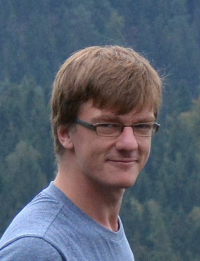
\includegraphics[width=\textwidth,keepaspectratio]{klindt.jpg}\vskip1ex
                            \textcontour{black}{\textbf{\scriptsize{Gary S Klindt}}}
                        \end{center}
                    \end{minipage} & \begin{minipage}{.22\paperwidth}
                        \begin{center}
                            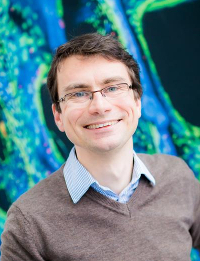
\includegraphics[width=\textwidth,keepaspectratio]{friedrich.jpg}\vskip1ex
                            \textcontour{black}{\textbf{\scriptsize{Dr Benjamin M Friedrich}}}
                        \end{center}
                    \end{minipage} & \begin{minipage}{.22\paperwidth}
                        \begin{center}
                            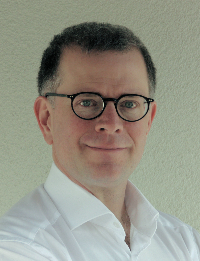
\includegraphics[width=\textwidth,keepaspectratio]{wagner.jpg}\vskip1ex
                            \textcontour{black}{\textbf{\scriptsize{Prof Dr Christian Wagner}}}
                        \end{center}
                    \end{minipage}
                \end{tabular}\\
                \vskip.5ex
                \hspace{3.6em}\textcontour{black}{\scriptsize{Max Planck Institute for the Physics of Complex Systems, Dresden}}\hfill\hfill
                \vskip5ex
                \textcontour{black}{
                Load Response of the Flagellar Beat\\
                \textit{GS Klindt\,\small{$^\star$}, CR\,\small{$^\star$}, C Wagner, and BM Friedrich}\\
                Phys. Rev. Lett. \textbf{117}, 258101\vspace{-.2em}\\
                {\scriptsize{($\star$ equal contribution)}}}
            \end{center}
            \vfill
        \end{frame}


\section{}
    \subsection{}
        \begin{frame}
            \frametitle{\Large{The eukaryotic flagellum:}\\\small{a very complex machine on a very small scale}}
            \vskip4ex
            \begin{center}
                \displayimage{black}{white}{0.9\textwidth}{2pt}{.2ex}{\vfill}{}{\includegraphics[width=\textwidth,keepaspectratio]{motivation.pdf}}{}
            \end{center}
            \vskip4ex
            \hfill\textcontour{black}{\textbf{\Large{How does it perform under load?}}}\hspace{3.5ex}\,\\
            \vskip8ex
            \begin{center}
                \textcontour{black}{\scriptsize{electron micrograph taken from Pazour et al., \textit{Proteomic analysis of a eukaryotic cilium}, J Cell Biol. \textbf{170}(1):103-13 (2005)}}
            \end{center}
            \vfill
        \end{frame}


\section{}
    \subsection{}
        \begin{frame}
            \frametitle{\Large{Holographic optical tweezers:}\\\small{contactless fixation and force sensing capabilities}}
            \begin{center}
                \begin{tabular}{ccc}
                    \begin{minipage}{.1\paperwidth}\,\end{minipage} & 
                    \begin{minipage}{.32\paperwidth}
                        \begin{center}
                            \displayimage{black}{white}{\textwidth}{2pt}{.2ex}{\vfill}{}{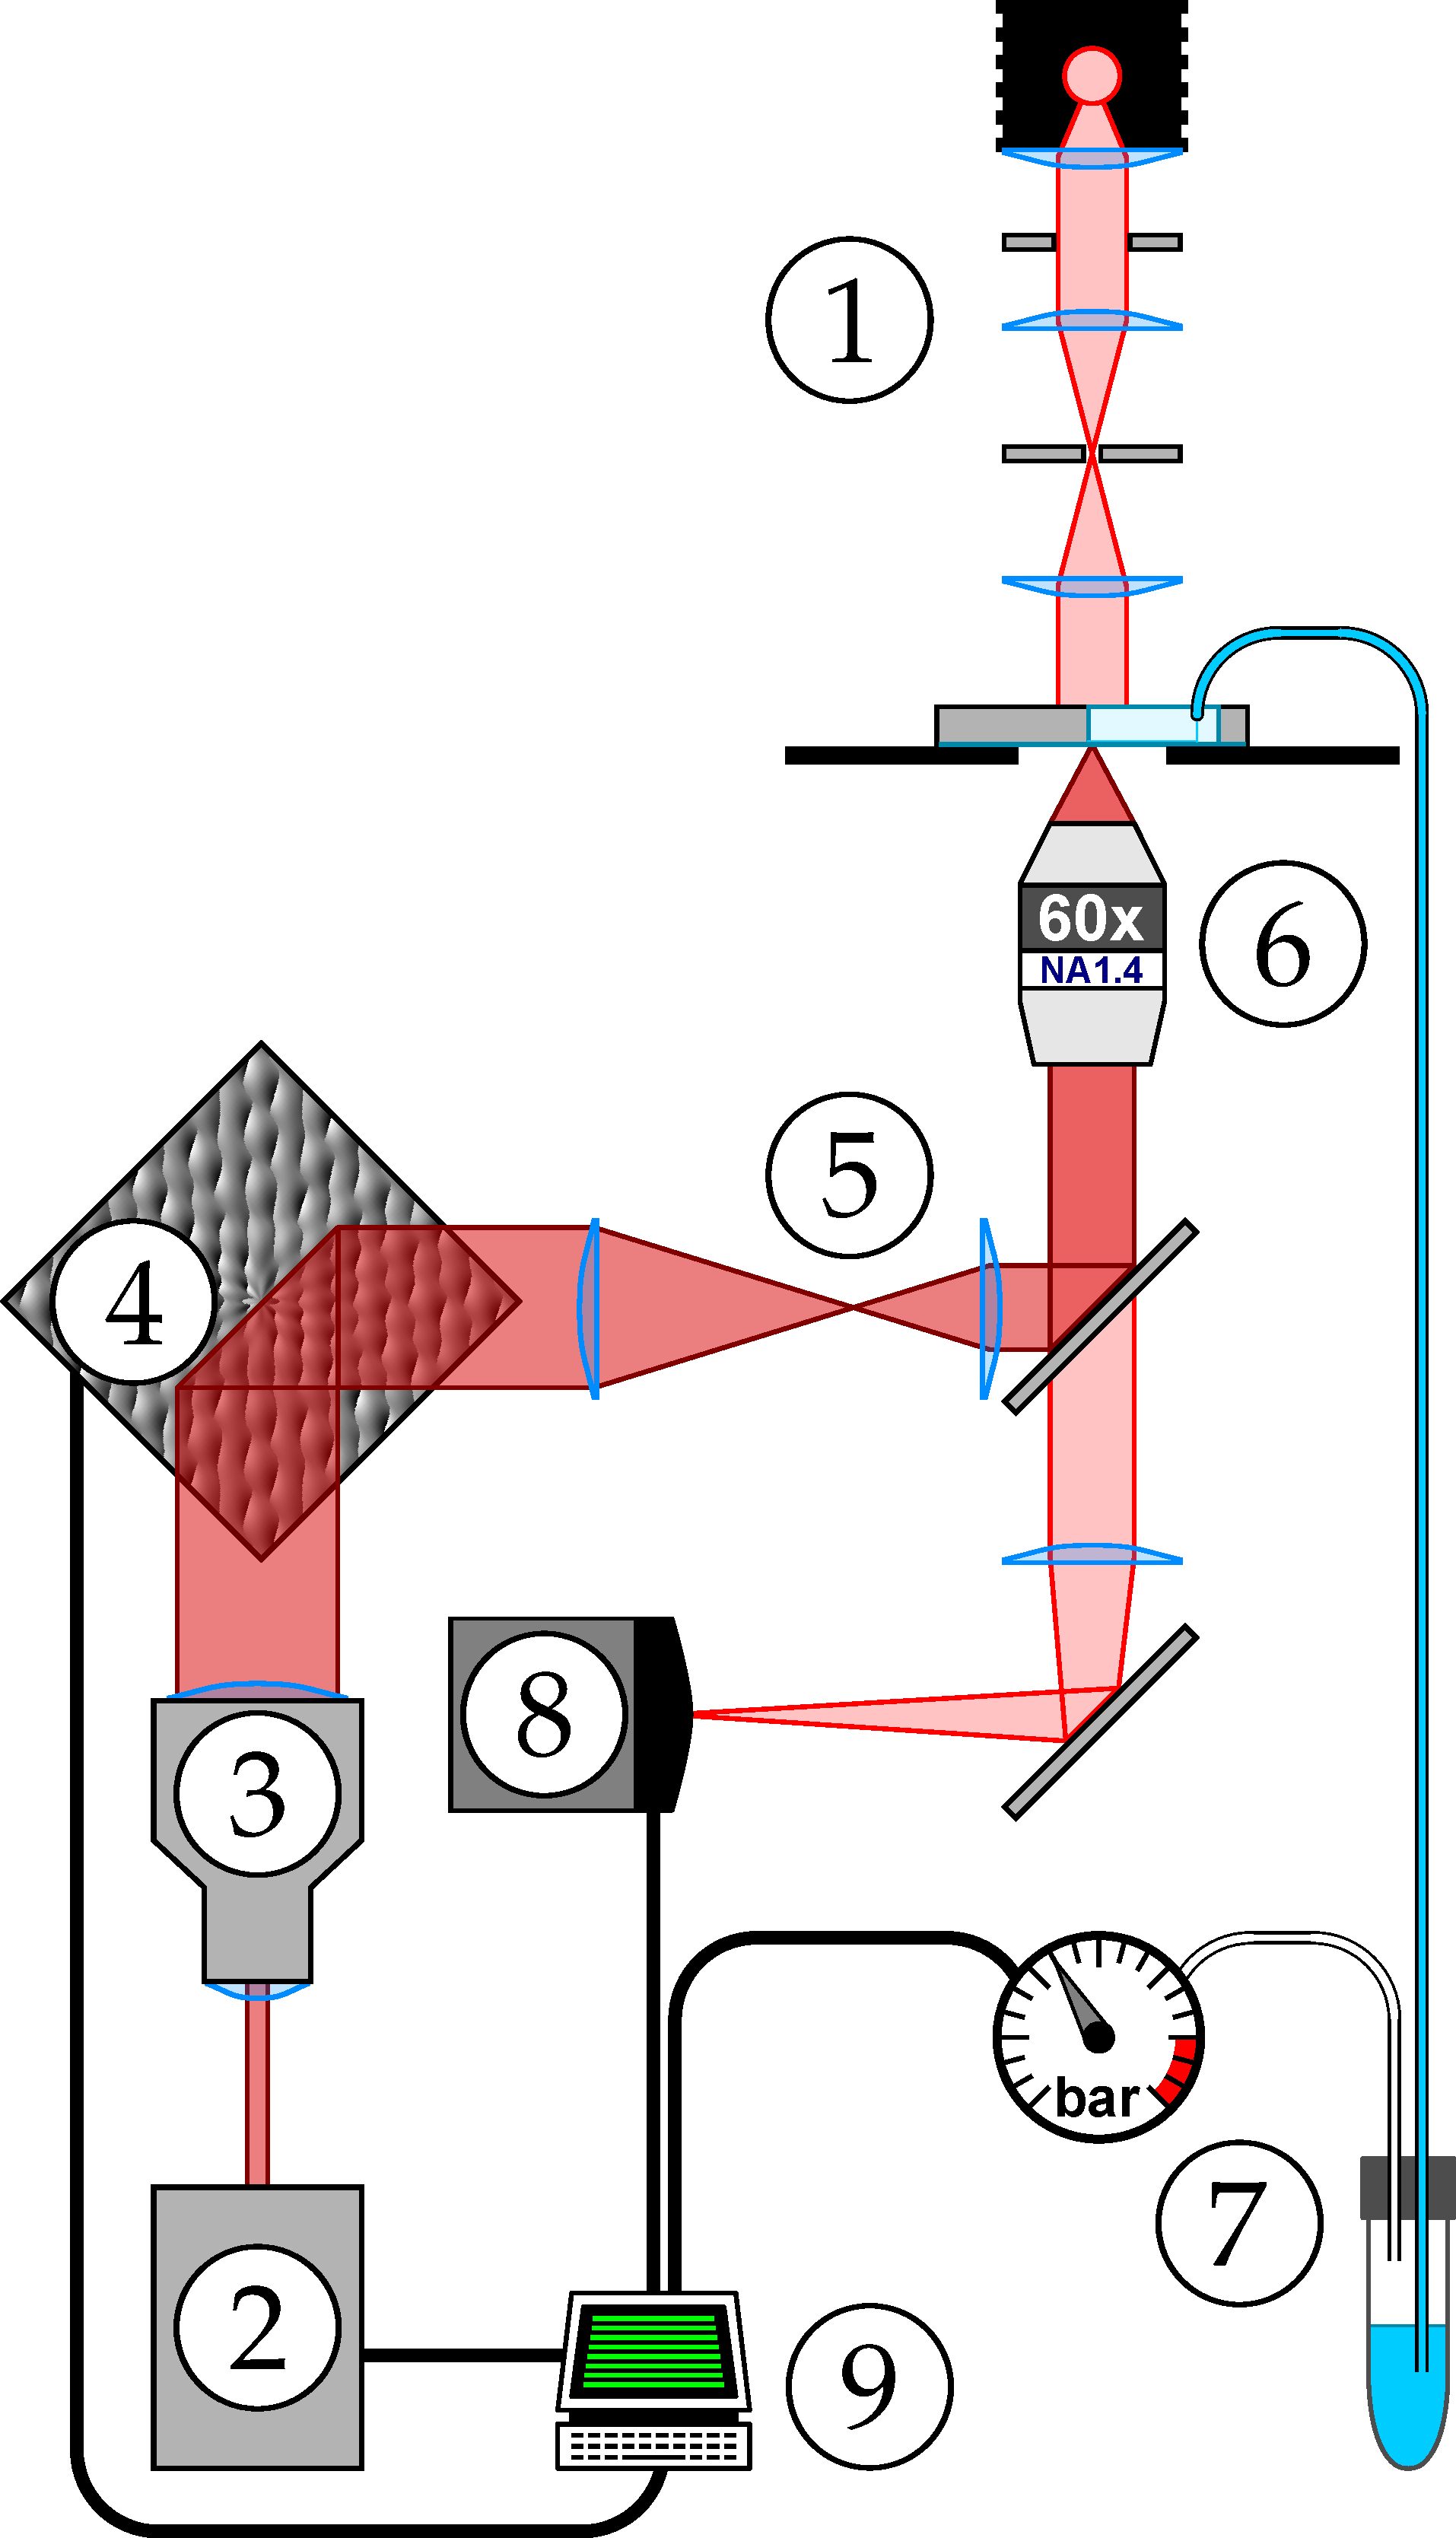
\includegraphics[width=\textwidth,keepaspectratio]{optical_tweezers.pdf}}{}\vskip2ex
                        \end{center}
                    \end{minipage} & \begin{minipage}{.44\paperwidth}
                        \begin{center}
                            \small{
                                \begin{enumerate}
                                    \item \textcontour{black}{custom-made Köhler illumination}
                                    \item \textcontour{black}{Nd:YAG laser, 1064\,nm 1.5\,W}
                                    \item \textcontour{black}{8$\times$ beam expander}
                                    \item \textcontour{black}{phase modulator (PAL-SLM)}
                                    \item \textcontour{black}{2$\times$ telescope}
                                    \item \textcontour{black}{60$\times$ oil-immersion objective, NA 1.4}
                                    \item \textcontour{black}{pressure controller}
                                    \item \textcontour{black}{high-speed camera}
                                    \item \textcontour{black}{PC}
                                \end{enumerate}
                            }
                        \end{center}
                    \end{minipage}
                \end{tabular}
            \end{center}
            \vfill
        \end{frame}


\section{}
    \subsection{}
        \begin{frame}
            \frametitle{\Large{Reliable orientation} \small{of optically trapped \textit{Chlamydomonas reinhardtii}}\\\Large{is impossible}}
            \begin{center}
%                   \displayimage{black}{white}{0.6\textwidth}{2pt}{.2ex}{\vfill}{}{\includegraphics[width=\textwidth,keepaspectratio]{swimming_in_an_optical_trap.pdf}}{}\vskip2ex
                \begin{tabular}{cc}
                    \begin{minipage}{.48\paperwidth}
                        \begin{center}
                            \displayimage{black}{white}{\textwidth}{2pt}{.2ex}{\vfill}{}{\includegraphics[width=\textwidth,keepaspectratio]{swimming_in_an_optical_trap.pdf}}{}\vskip2ex
                        \end{center}
                    \end{minipage} & \begin{minipage}{.36\paperwidth}
                        \begin{center}
                            \vspace{.7em}\movie[width=\textwidth,poster,autostart,showcontrols,loop,externalviewer]{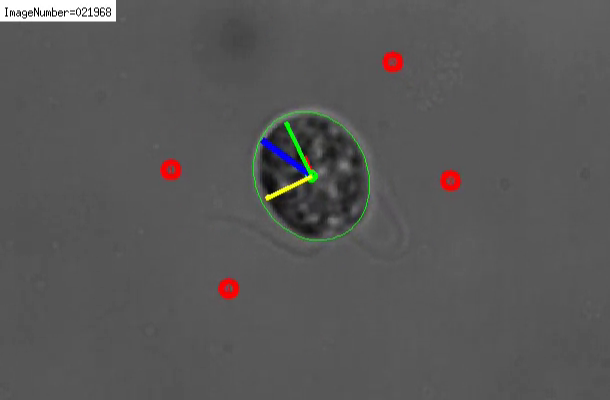
\includegraphics[width=\textwidth,keepaspectratio]{chlamy_trap_60x_1kHz_25fps.png}}{chlamy_trap_60x_1kHz_25fps.webm}
                        \end{center}
                    \end{minipage}
                \end{tabular}
                \vskip2ex
%                 \movie[width=0.5\textwidth,poster,autostart,showcontrols,loop,externalviewer]{\includegraphics[width=0.5\textwidth,keepaspectratio]{cr+ot.png}}{cr+ot.avi}
                \small{
                    \begin{itemize}
                        \item \textcontour{black}{cell rotates out of the focal plane}
                        \item \textcontour{black}{optical forces just strong enough for trapping under no flow conditions}
                    \end{itemize}
                }
            \end{center}
            \vfill
        \end{frame}


\section{}
    \subsection{}
        \begin{frame}
            \frametitle{\Large{Micropipettes:}\\\small{strong fixation and reliable orientation}}
            \begin{center}
                \displayimage{black}{white}{0.9\textwidth}{2pt}{.2ex}{\vfill}{}{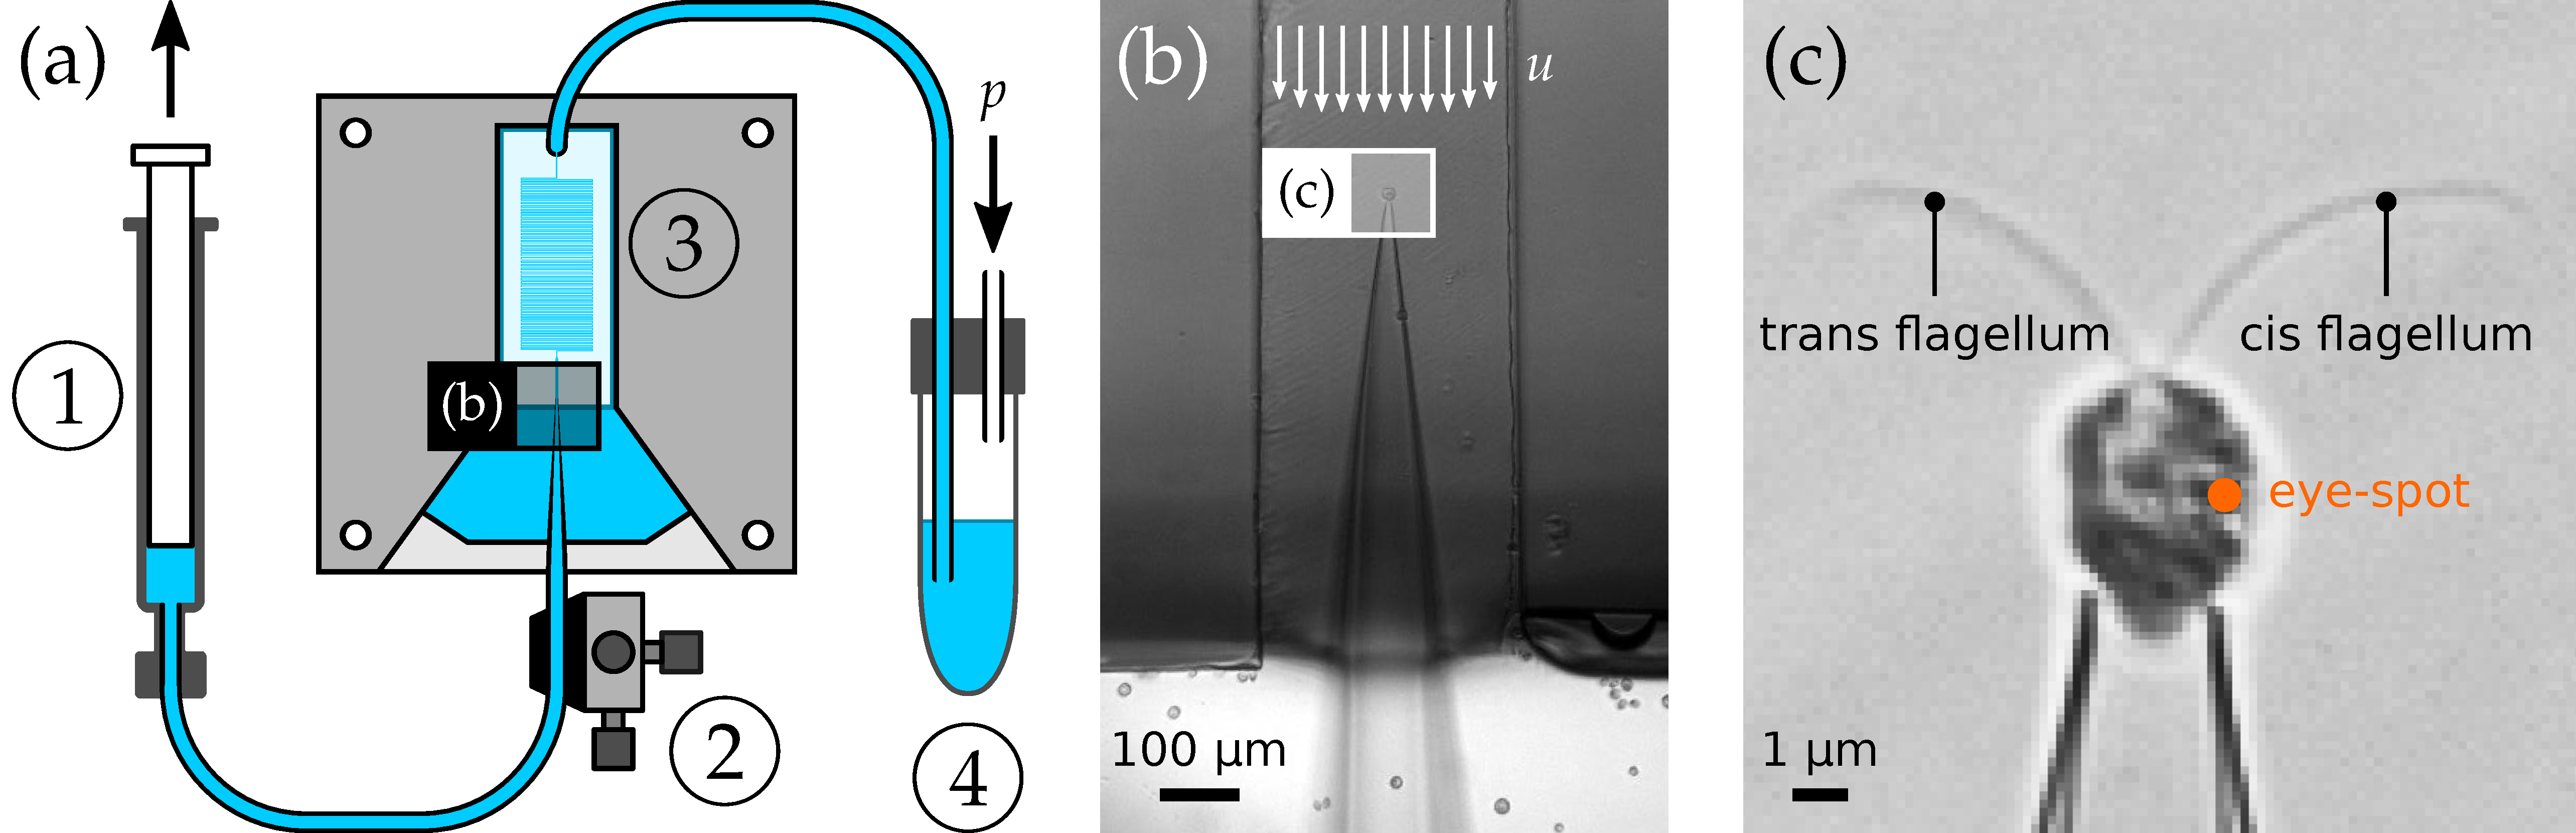
\includegraphics[width=\textwidth,keepaspectratio]{setup_single.pdf}}{}\vskip2ex
                \small{
                    \begin{enumerate}
                        \item \textcontour{black}{manually operated syringe}
                        \item \textcontour{black}{custom-made translational and rotational holder for micropipettes}
                        \item \textcontour{black}{microfluidics chip (pre-resistor channel and sample channel, sequential)}
                        \item \textcontour{black}{fluid reservoir to control the flow speed by means of a pressure device}
                    \end{enumerate}
                }
            \end{center}
            \vfill
        \end{frame}


\section{}
    \subsection{}
        \begin{frame}
            \frametitle{\small{Fully automated measurements are possible due to}\\\Large{device control toolboxes}}
            \begin{center}
                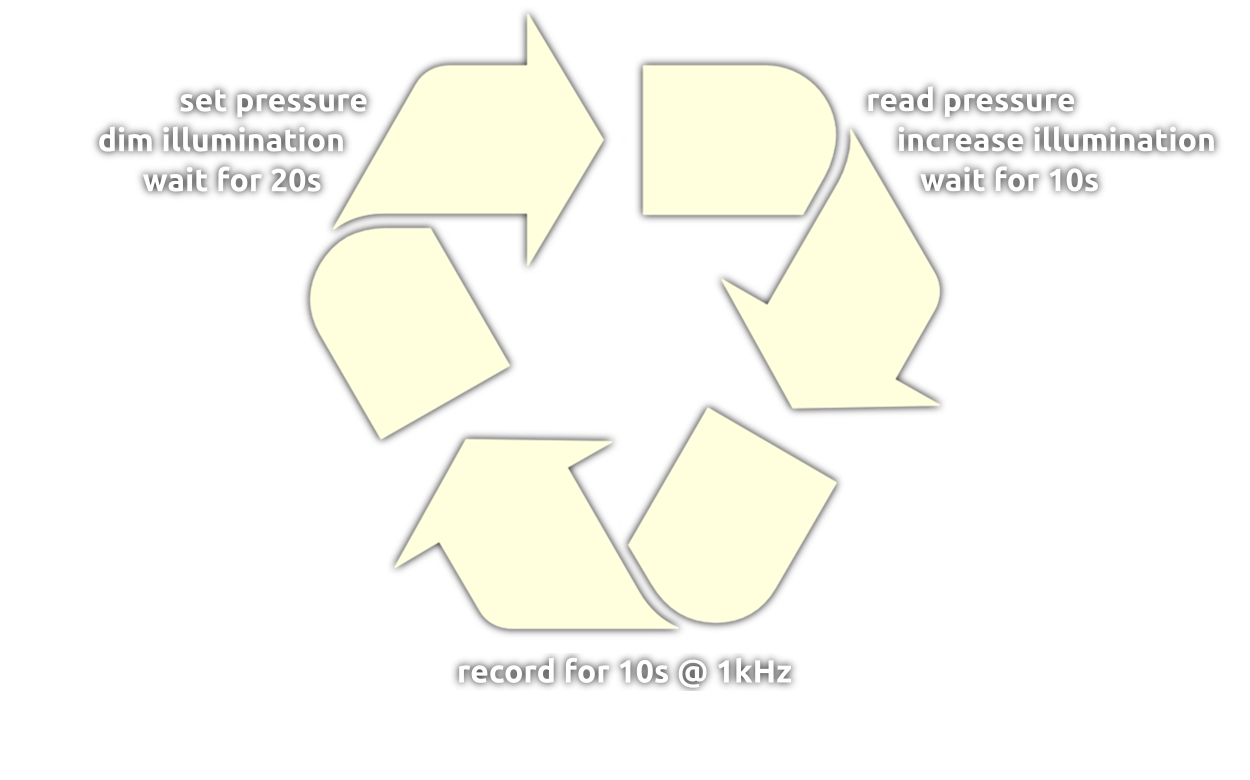
\includegraphics[width=0.8\textwidth,keepaspectratio]{messprotokoll.png}
            \end{center}
            \vfill
        \end{frame}


\section{}
    \subsection{}
        \begin{frame}
            \frametitle{\Large{High precision flagellar tracking}\\\small{reveals full dynamics of flagellar beating}}
            \begin{center}
                \displayimage{black}{white}{0.9\textwidth}{2pt}{.2ex}{\vfill}{}{\includegraphics[width=\textwidth,keepaspectratio]{track_flagella.pdf}}{}\vskip2ex
            \end{center}
            \vfill
        \end{frame}


\section{}
    \subsection{}
        \begin{frame}
            \frametitle{\small{High-dimensional measurement data is reduced to a two-dimensional}\\\Large{limit cycle representation}}
            \begin{center}
                \displayimage{black}{white}{0.9\textwidth}{2pt}{.2ex}{\vfill}{}{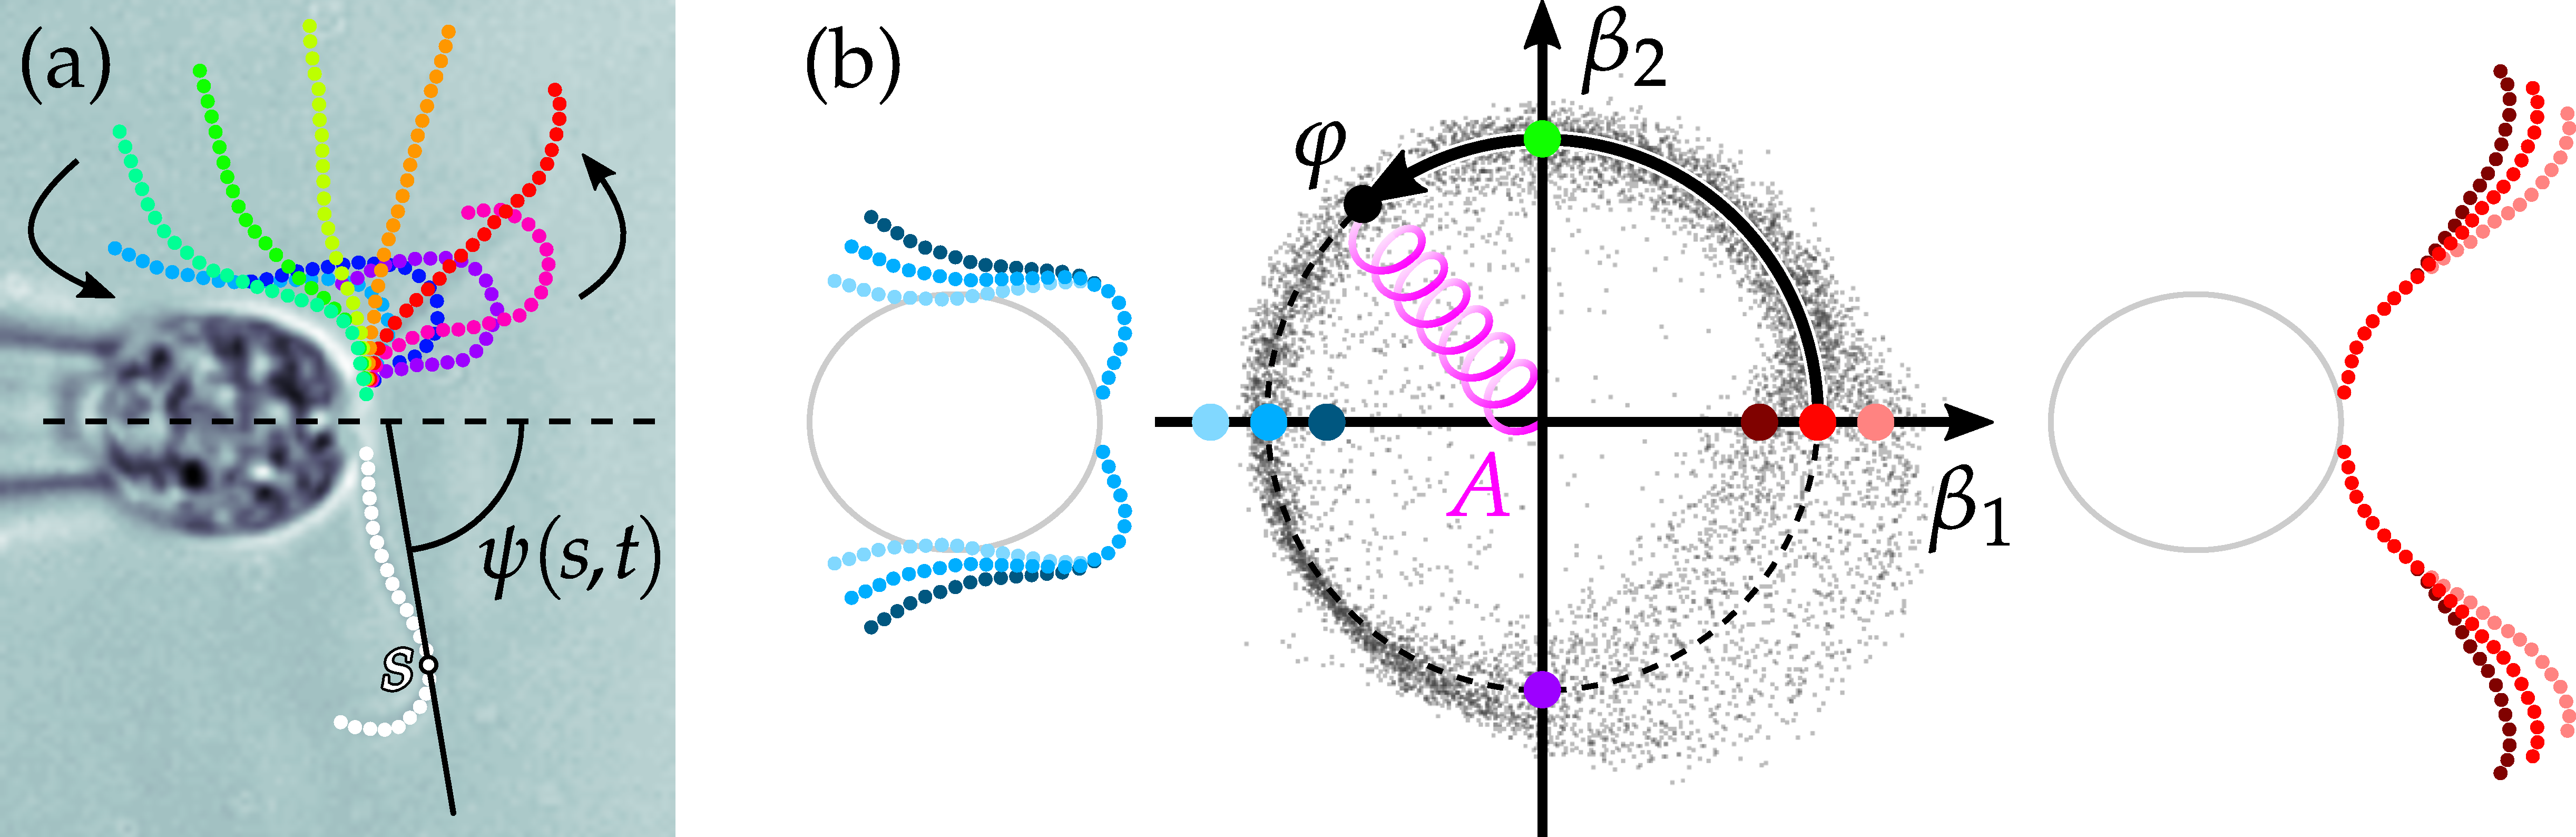
\includegraphics[width=\textwidth,keepaspectratio]{limit_cycle_representation.pdf}}{}\vskip2ex
                \small{
                    \begin{itemize}
                        \item \textcontour{black}{tangent angle representation $\psi\left(s, t\right)$ for flagellar point $s=1\dots S$ at times $t=1\dots T$}
                        \item \textcontour{black}{principle component analysis: $\psi\left(s, t\right) = \sum\limits_{n=1}^S\beta_n\left(t\right)\tilde{\psi}_n\left(s\right)$}
                        \item \textcontour{black}{$Z\left(t\right) = \beta_1\left(t\right) + \textrm{i}\beta_2\left(t\right) = A\left(t\right)\exp\left(\textrm{i}\varphi\left(t\right)\right)$}
                    \end{itemize}
                }
            \end{center}
            \vfill
        \end{frame}


\section{}
    \subsection{}
        \begin{frame}
            \frametitle{\Large{The flagellar load response} \small{is characterised by\newline the amplitude susceptibility $\chi_{A}$ and the phase speed susceptibility $\chi_{\dot{\varphi}}$}}
            \begin{center}
                \displayimage{black}{white}{0.9\textwidth}{2pt}{.2ex}{\vfill}{}{\includegraphics[width=\textwidth,keepaspectratio]{a_phi__v__u.pdf}}{}\vskip2ex
                \large\textcontour{black}{$\frac{A}{A_0}\approx 1 + \chi_{A}\cdot u\quad\textsf{and}\quad\frac{\dot{\varphi}}{\dot{\varphi}_0}\approx 1 + \chi_{\dot{\varphi}}\cdot u$}
            \end{center}
            \vfill
        \end{frame}


\section{}
    \subsection{}
        \begin{frame}
            \frametitle{\Large{The flagellar load response} \small{is highly phase-dependent}}
            \begin{center}
                \displayimage{black}{white}{0.9\textwidth}{2pt}{.2ex}{\vfill}{}{\includegraphics[width=\textwidth,keepaspectratio]{chi__v__phi.pdf}}{}\vskip2ex
                \small{
                    \begin{itemize}
                        \item \textcontour{black}{during the recovery stroke, the flagella are closer to the cell body}
                        \item \textcontour{black}{the recovery stroke slows down}
                        \item \textcontour{black}{the power stroke speeds up}
                    \end{itemize}
                }
            \end{center}
            \vfill
        \end{frame}


\section{}
    \subsection{}
        \begin{frame}
            \frametitle{\Large{The frequency response of the flagellar beat}\\\small{reveals dynamic beating modes and shows hysteresis}}
            \begin{center}
                \displayimage{black}{white}{0.9\textwidth}{2pt}{.2ex}{\vfill}{}{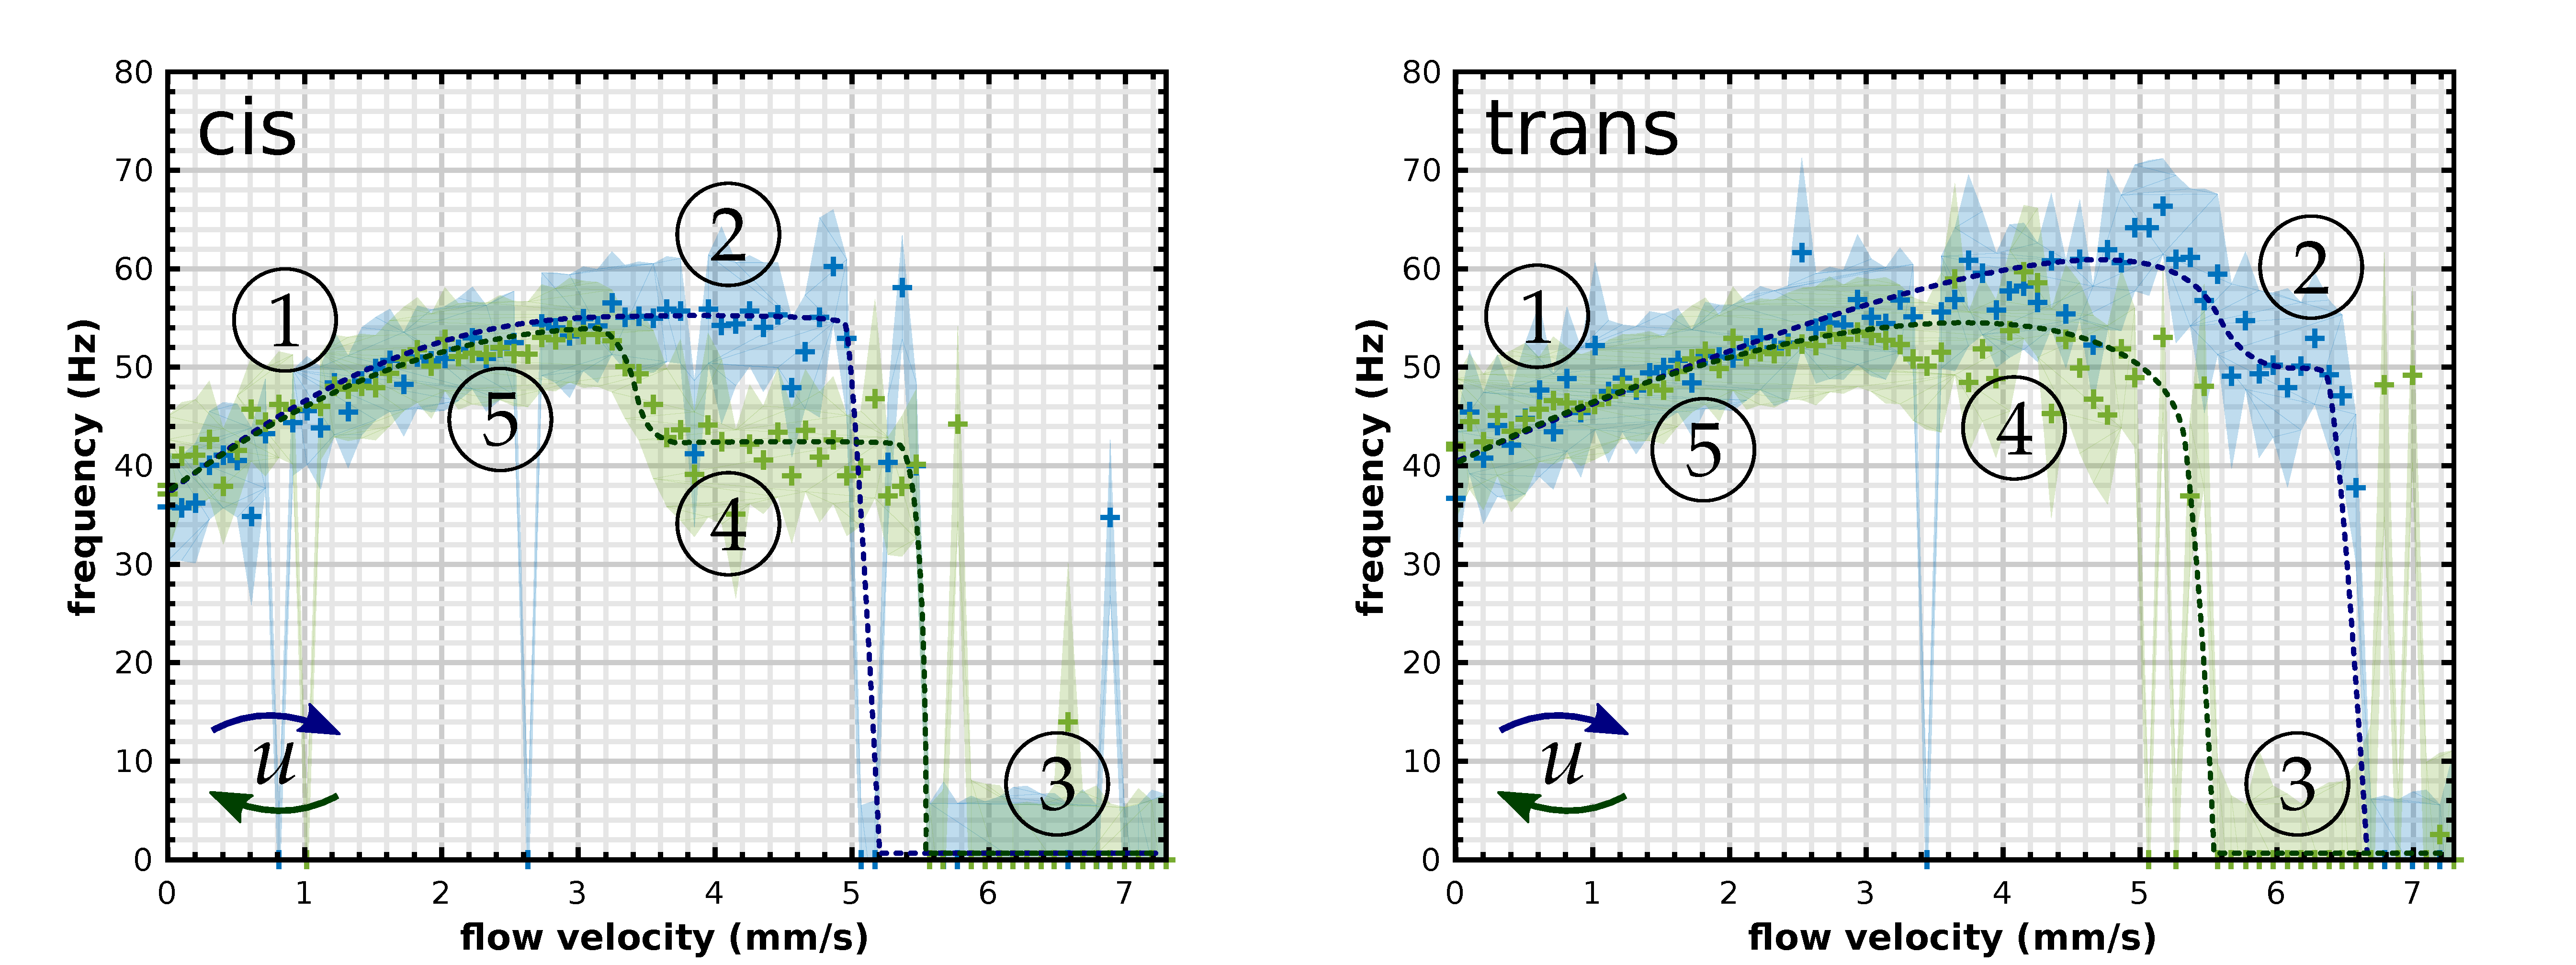
\includegraphics[width=\textwidth,keepaspectratio]{20160217_064935_fine_frequency__v__flow_velocity__cis_trans_height_main.pdf}}{}\vskip2ex
                \small{
                    \begin{itemize}
                        \item \textcontour{black}{low load: almost linear frequency response}
                        \item \textcontour{black}{intermediate load: chiral beating and tremor-like beating}
                        \item \textcontour{black}{high load: stalling}
                    \end{itemize}
%                     \begin{enumerate}
%                         \item \textcontour{black}{low external load: almost linear frequency response}
%                         \item \textcontour{black}{intermediate external load: tremor-like beating}
%                         \item \textcontour{black}{high external load: stalling showing almost no hysteresis (cis) and strong hysteresis (trans)}
%                         \item \textcontour{black}{intermediate external load: chiral beating (cis) and tremor-like beating (trans)}
%                         \item \textcontour{black}{low external load: linear frequency response (identical to 1.)}
%                     \end{enumerate}
                }
            \end{center}
            \vfill
        \end{frame}


\section{}
    \subsection{}
        \begin{frame}
            \frametitle{\Large{Flagellar synchronisation changes with external load}\\\small{but does not switch from in-phase to anti-phase}}
            \begin{center}
                \displayimage{black}{white}{0.5\textwidth}{2pt}{.2ex}{\vfill}{}{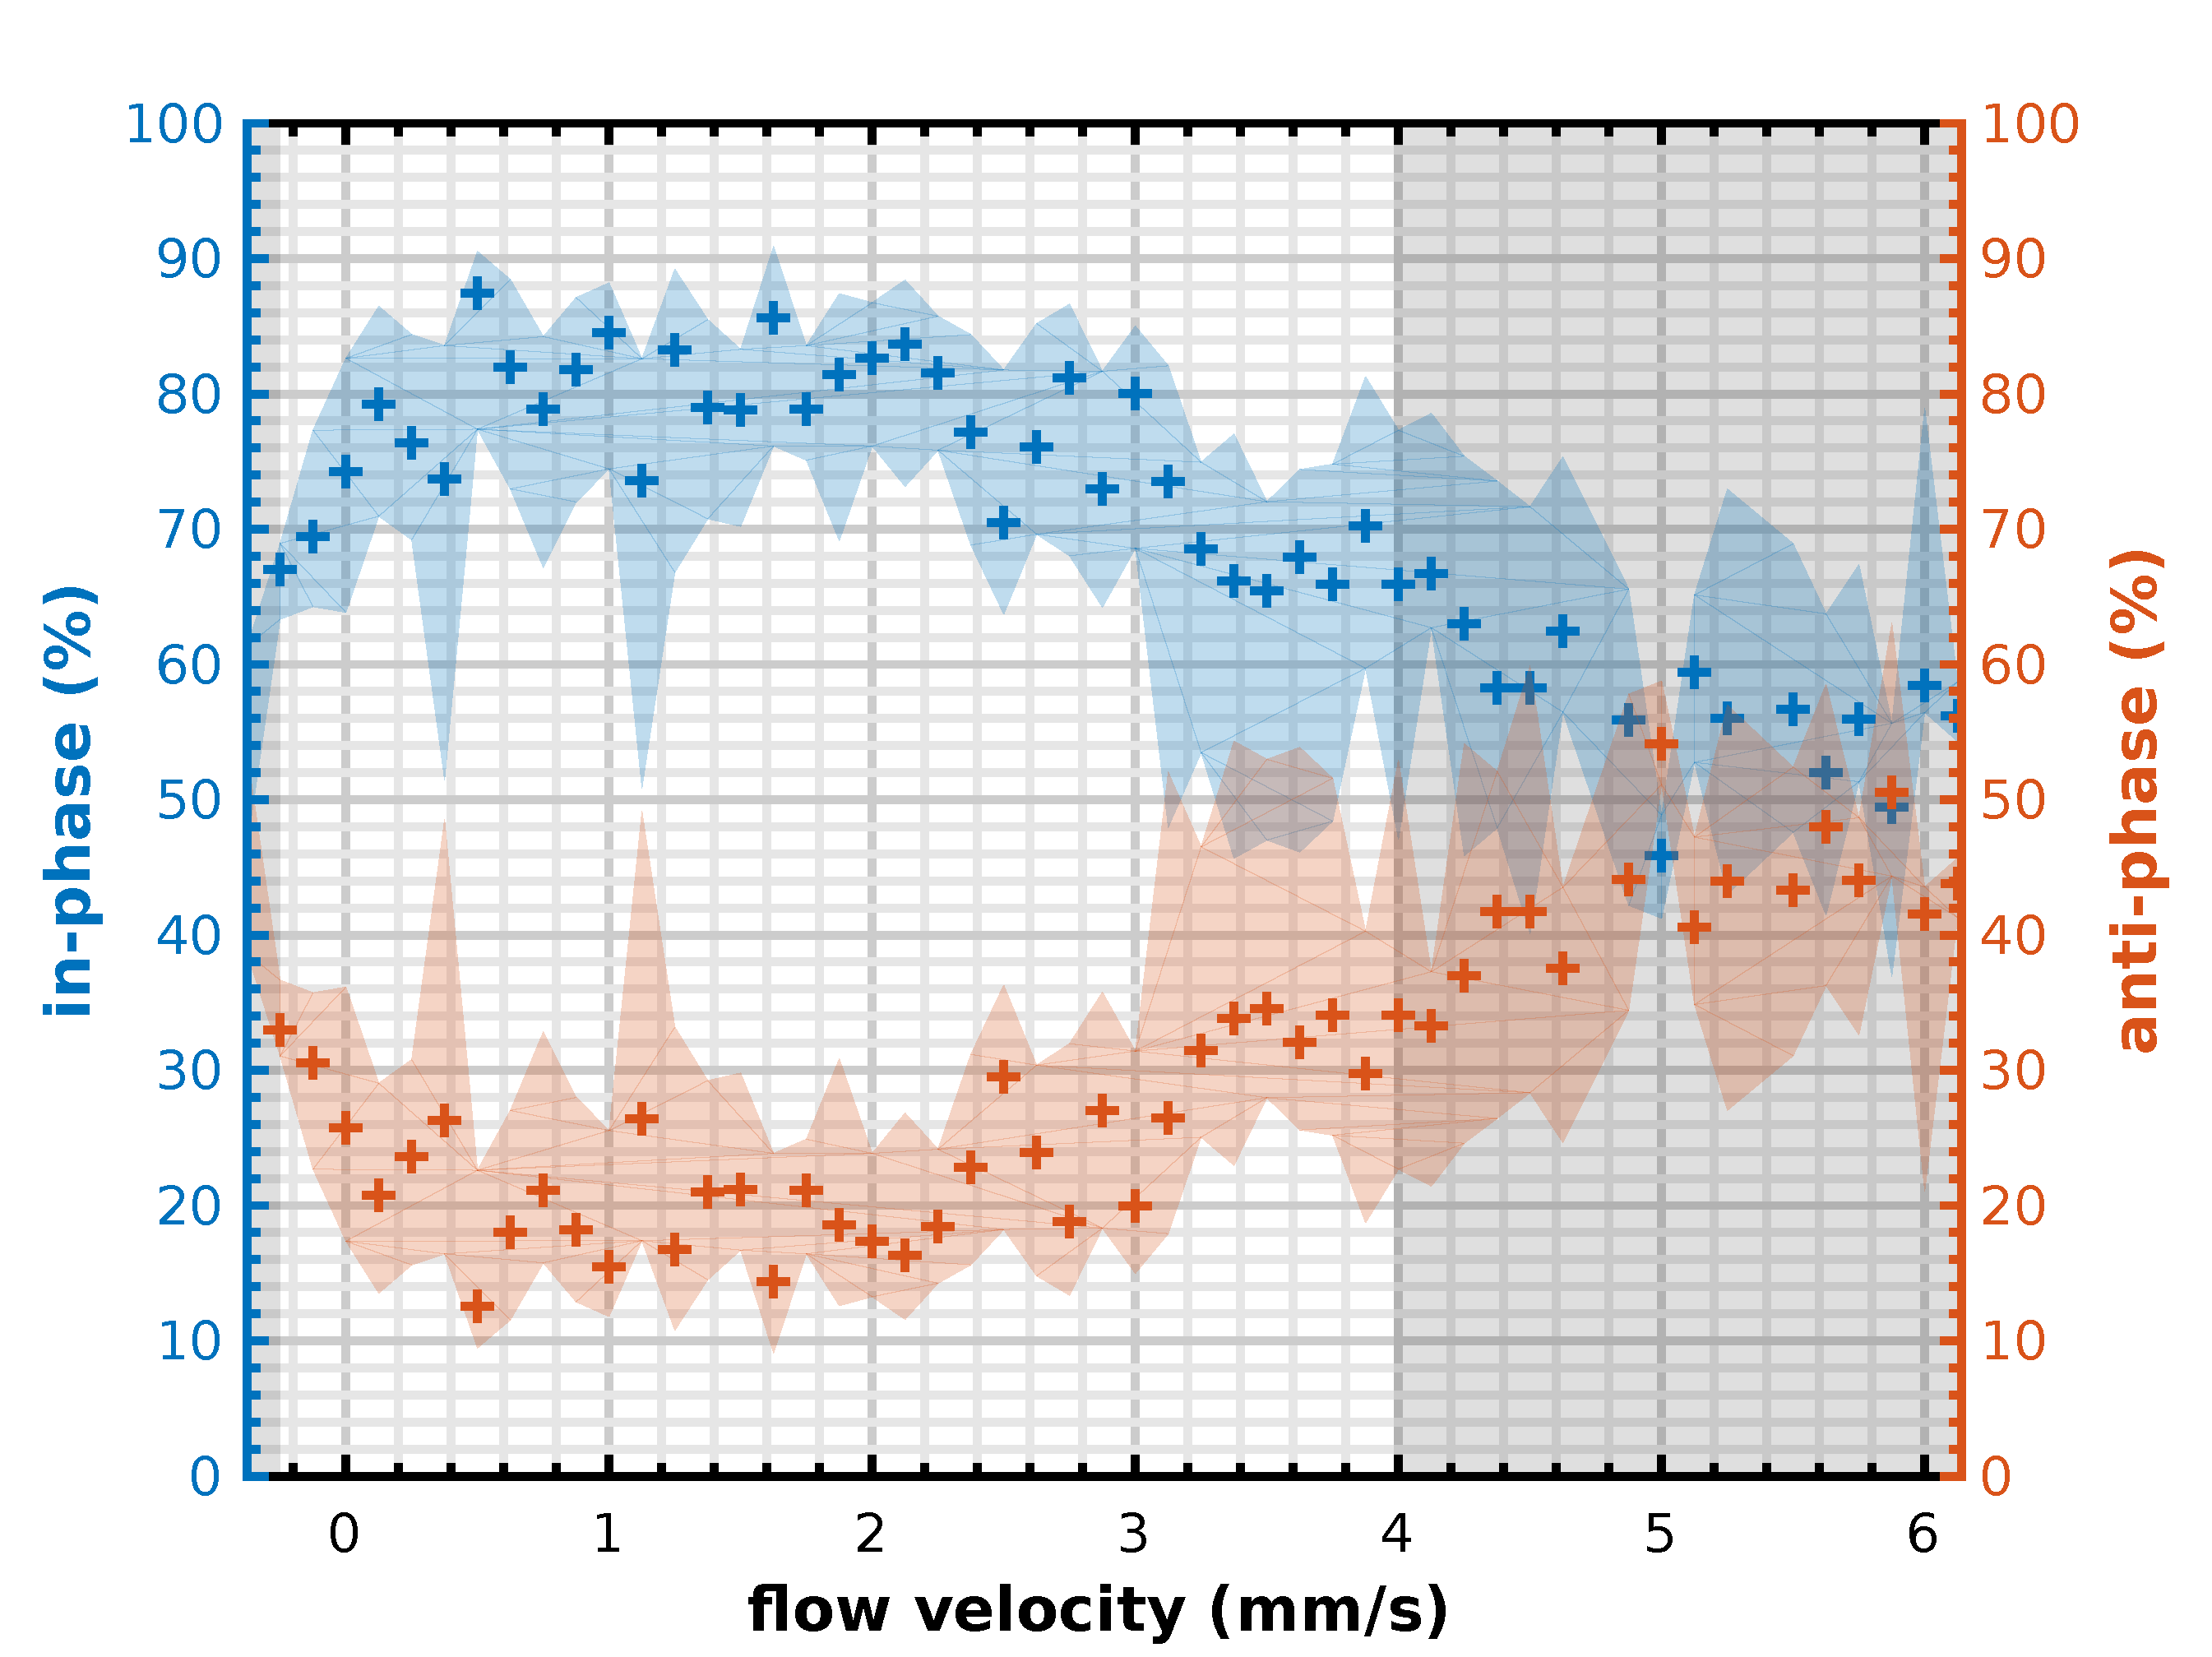
\includegraphics[width=\textwidth,keepaspectratio]{flagellar_distance__and__ip__and__ap__v__u.pdf}}{}\vskip2ex
                \small{
                    \begin{itemize}
                        \item \textcontour{black}{low positive load: almost no change in flagellar synchrony}
                        \item \textcontour{black}{intermediate positive load: reduced flagellar synchrony}
                        \item \textcontour{black}{negative load: loss of flagellar synchrony}
                    \end{itemize}
                }
            \end{center}
            \vfill
        \end{frame}


% \section{}
%     \subsection{}
%         \begin{frame}
%             \frametitle{\Large{stalling velocities}}
%             \begin{center}
%                 \displayimage{black}{white}{0.9\textwidth}{2pt}{.2ex}{\vfill}{}{\includegraphics[width=\textwidth,keepaspectratio]{cis_and_trans_to_and_from_stalling_all.pdf}}{}\vskip2ex
%             \end{center}
%             \vfill
%         \end{frame}
%         \begin{frame}
%             \frametitle{\Large{stalling velocities}}
%             \begin{center}
%                 \displayimage{black}{white}{0.9\textwidth}{2pt}{.2ex}{\vfill}{}{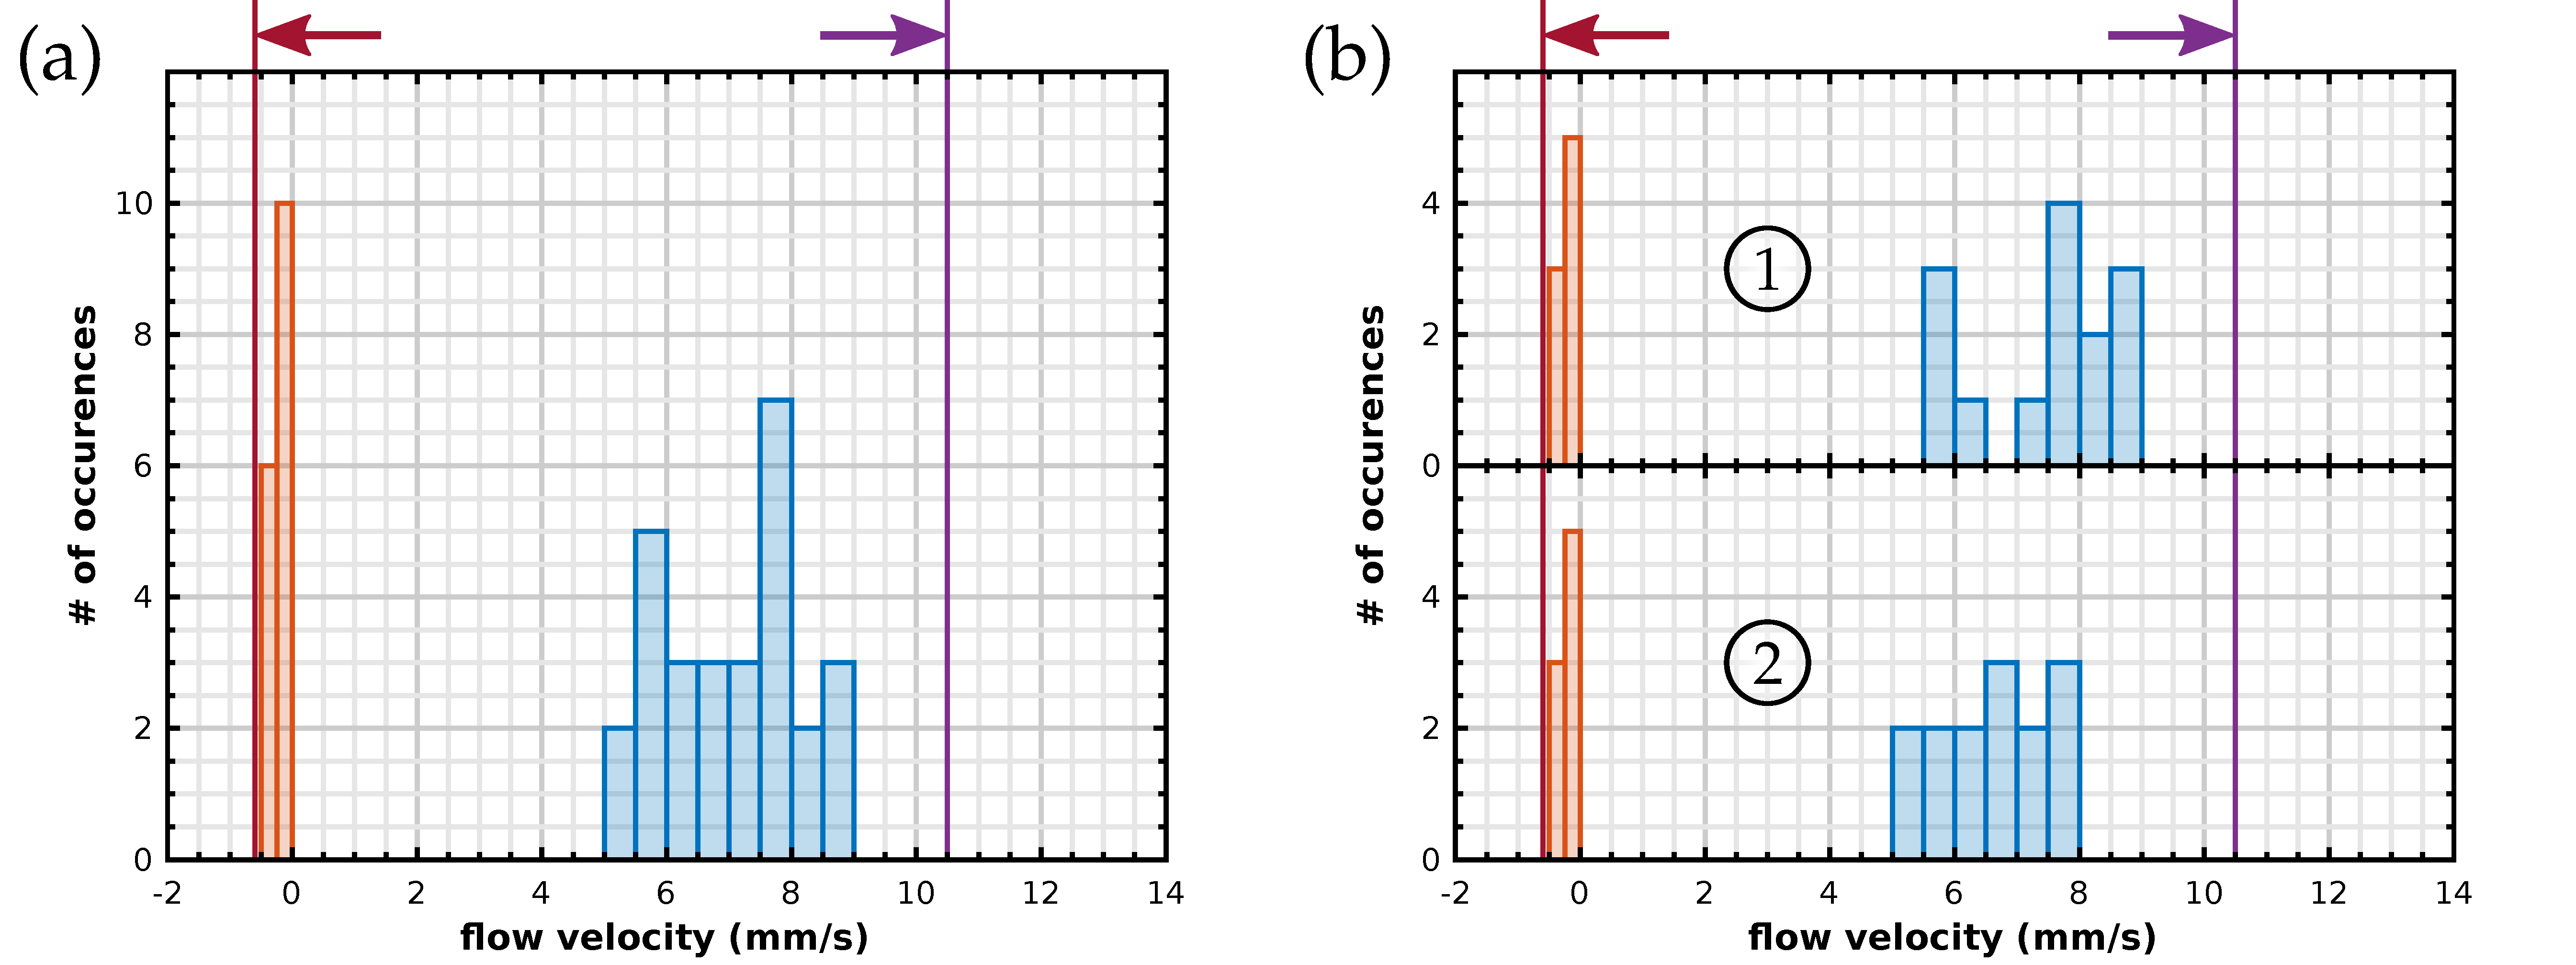
\includegraphics[width=\textwidth,keepaspectratio]{cis_and_trans_to_stalling_all.pdf}}{}\vskip2ex
%             \end{center}
%             \vfill
%         \end{frame}
%         \begin{frame}
%             \frametitle{\Large{stalling velocities}}
%             \begin{center}
%                 \displayimage{black}{white}{0.9\textwidth}{2pt}{.2ex}{\vfill}{}{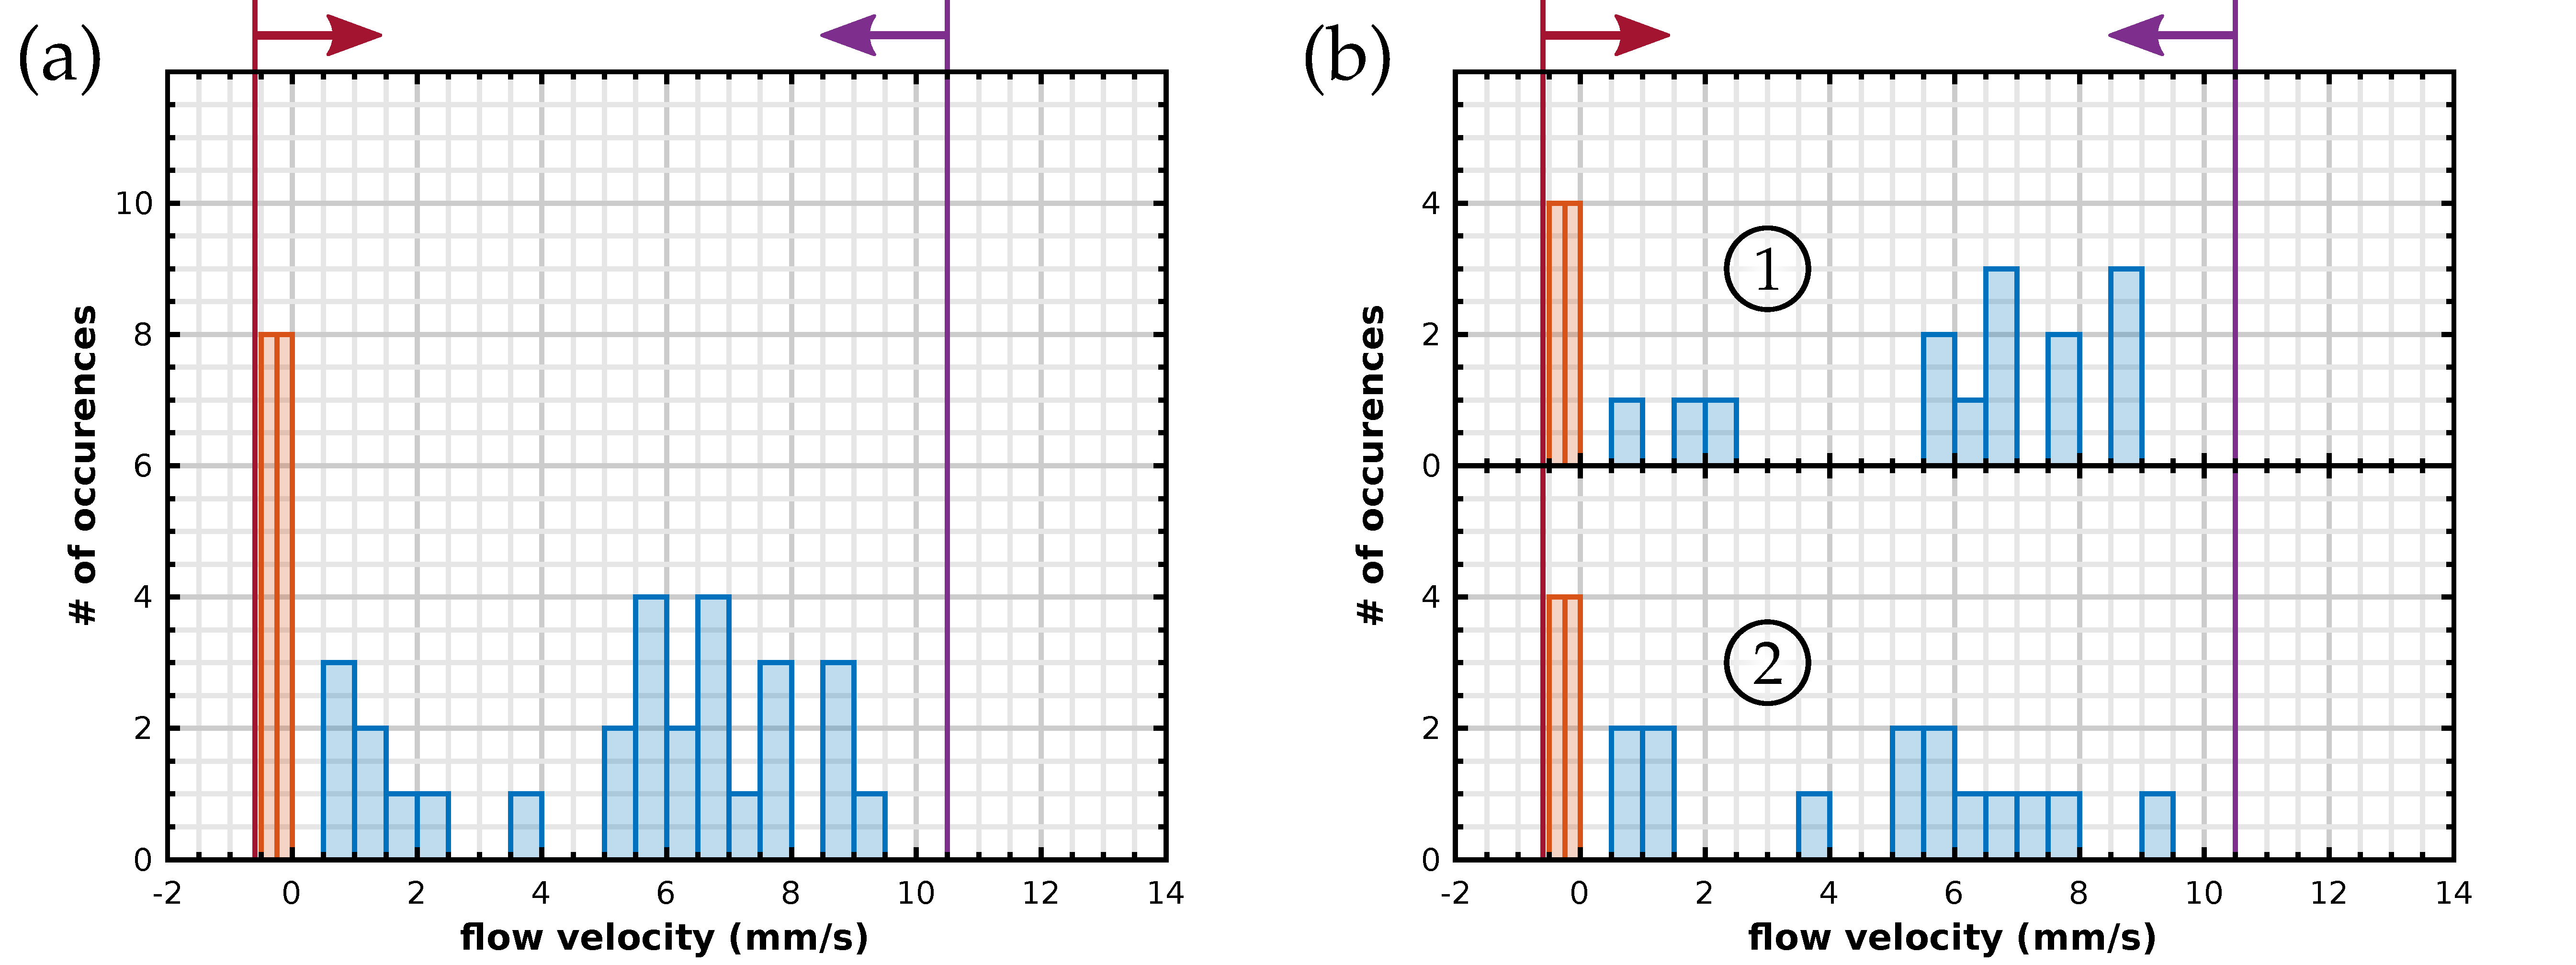
\includegraphics[width=\textwidth,keepaspectratio]{cis_and_trans_from_stalling_all.pdf}}{}\vskip2ex
%             \end{center}
%             \vfill
%         \end{frame}


% \section{}
%     \subsection{}
%         \begin{frame}
%             \frametitle{\Large{Different response of cis and trans flagellum}}
%             \begin{center}
%                 \displayimage{black}{white}{0.9\textwidth}{2pt}{.2ex}{\vfill}{}{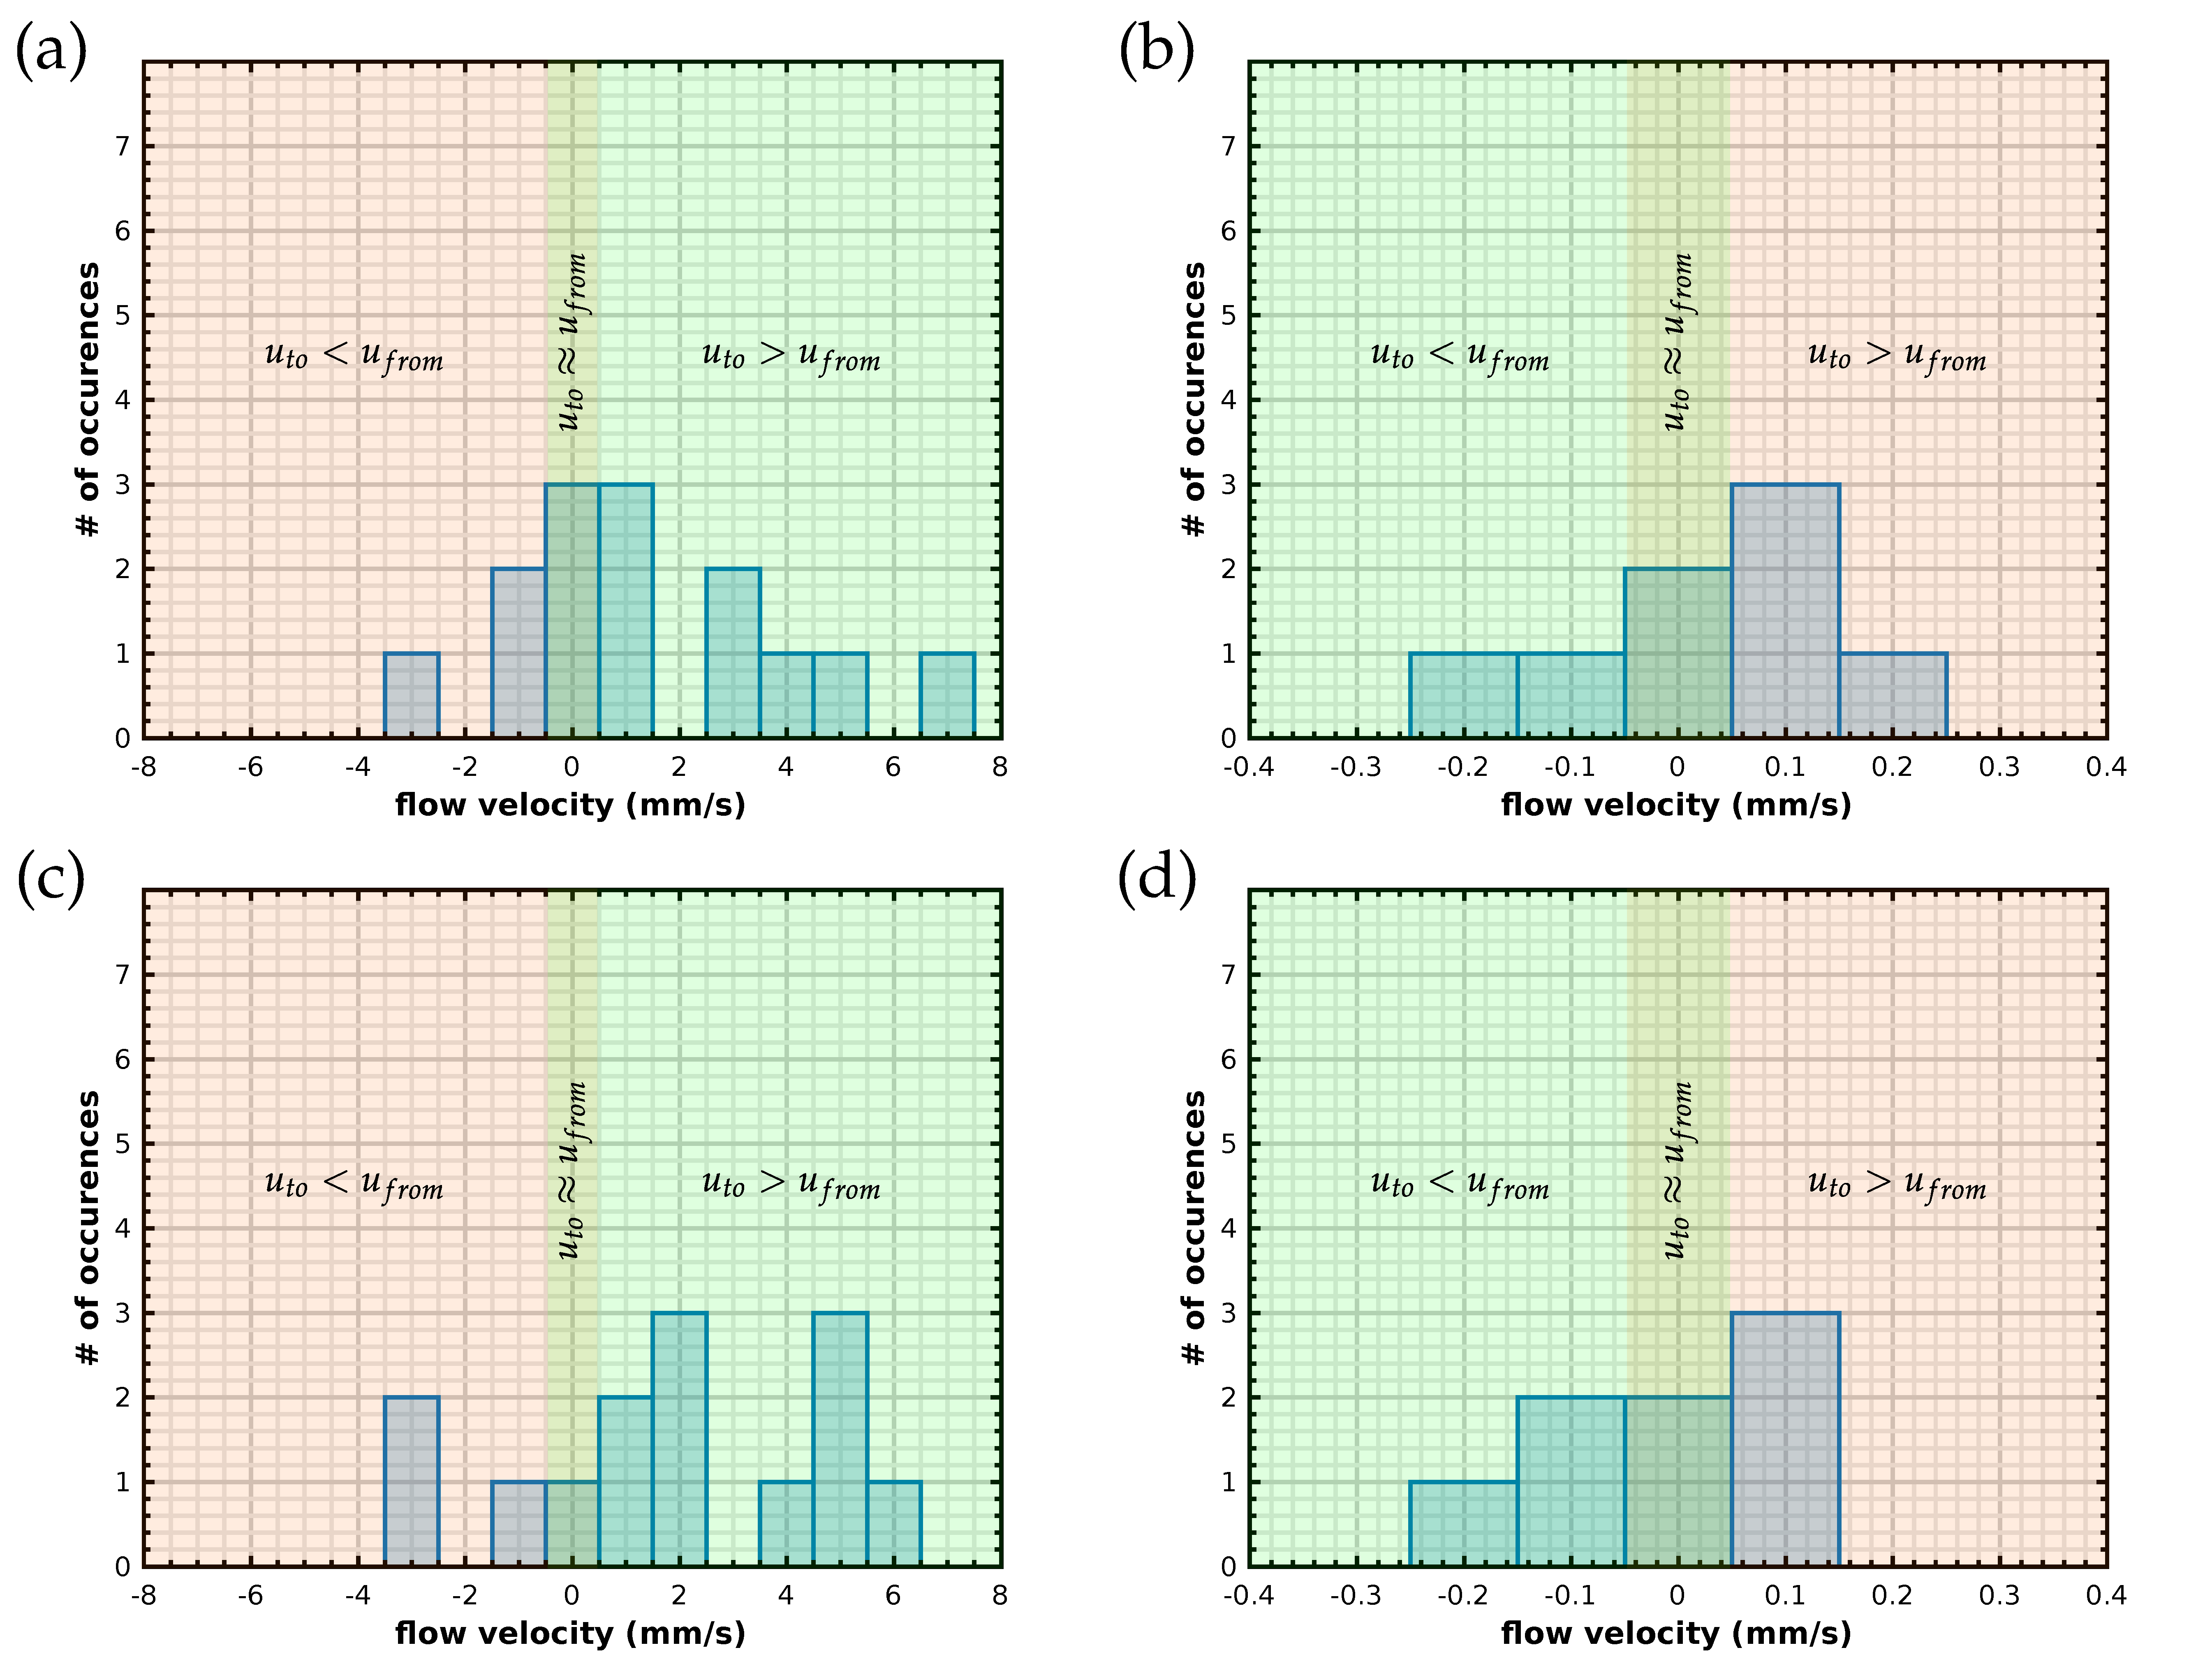
\includegraphics[width=\textwidth,keepaspectratio]{hysterese_in_stalling_velocities_to_and_from.pdf}}{}\vskip2ex
%             \end{center}
%             \vfill
%         \end{frame}


\section{}
    \subsection{}
        \begin{frame}
            \frametitle{\Large{Two dynamic modes of beating for positive load...}\\\small{(chiral and tremor-like beating)}}
            \vspace{1em}
            \begin{center}
                \movie[width=0.8\textwidth,poster,autostart,showcontrols,loop,externalviewer]{\includegraphics[width=0.8\textwidth,keepaspectratio]{supplemental_movie_S1.png}}{supplemental_movie_S1.mp4}\\\vskip3em
                \hfill\textcontour{black}{\textbf{\Large{...which do not exist for negative load}}}\hspace{3.5ex}\,\\\vskip1em
                \movie[width=0.8\textwidth,poster,autostart,showcontrols,loop,externalviewer]{\includegraphics[width=0.8\textwidth,keepaspectratio]{supplemental_movie_S2.png}}{supplemental_movie_S2.mp4}
            \end{center}
            \vfill
        \end{frame}
        \begin{frame}
            \frametitle{\Large{Different response of cis and trans flagellum}\\\small{to external load}}
            \begin{center}
                \displayimage{black}{white}{0.9\textwidth}{2pt}{.2ex}{\vfill}{}{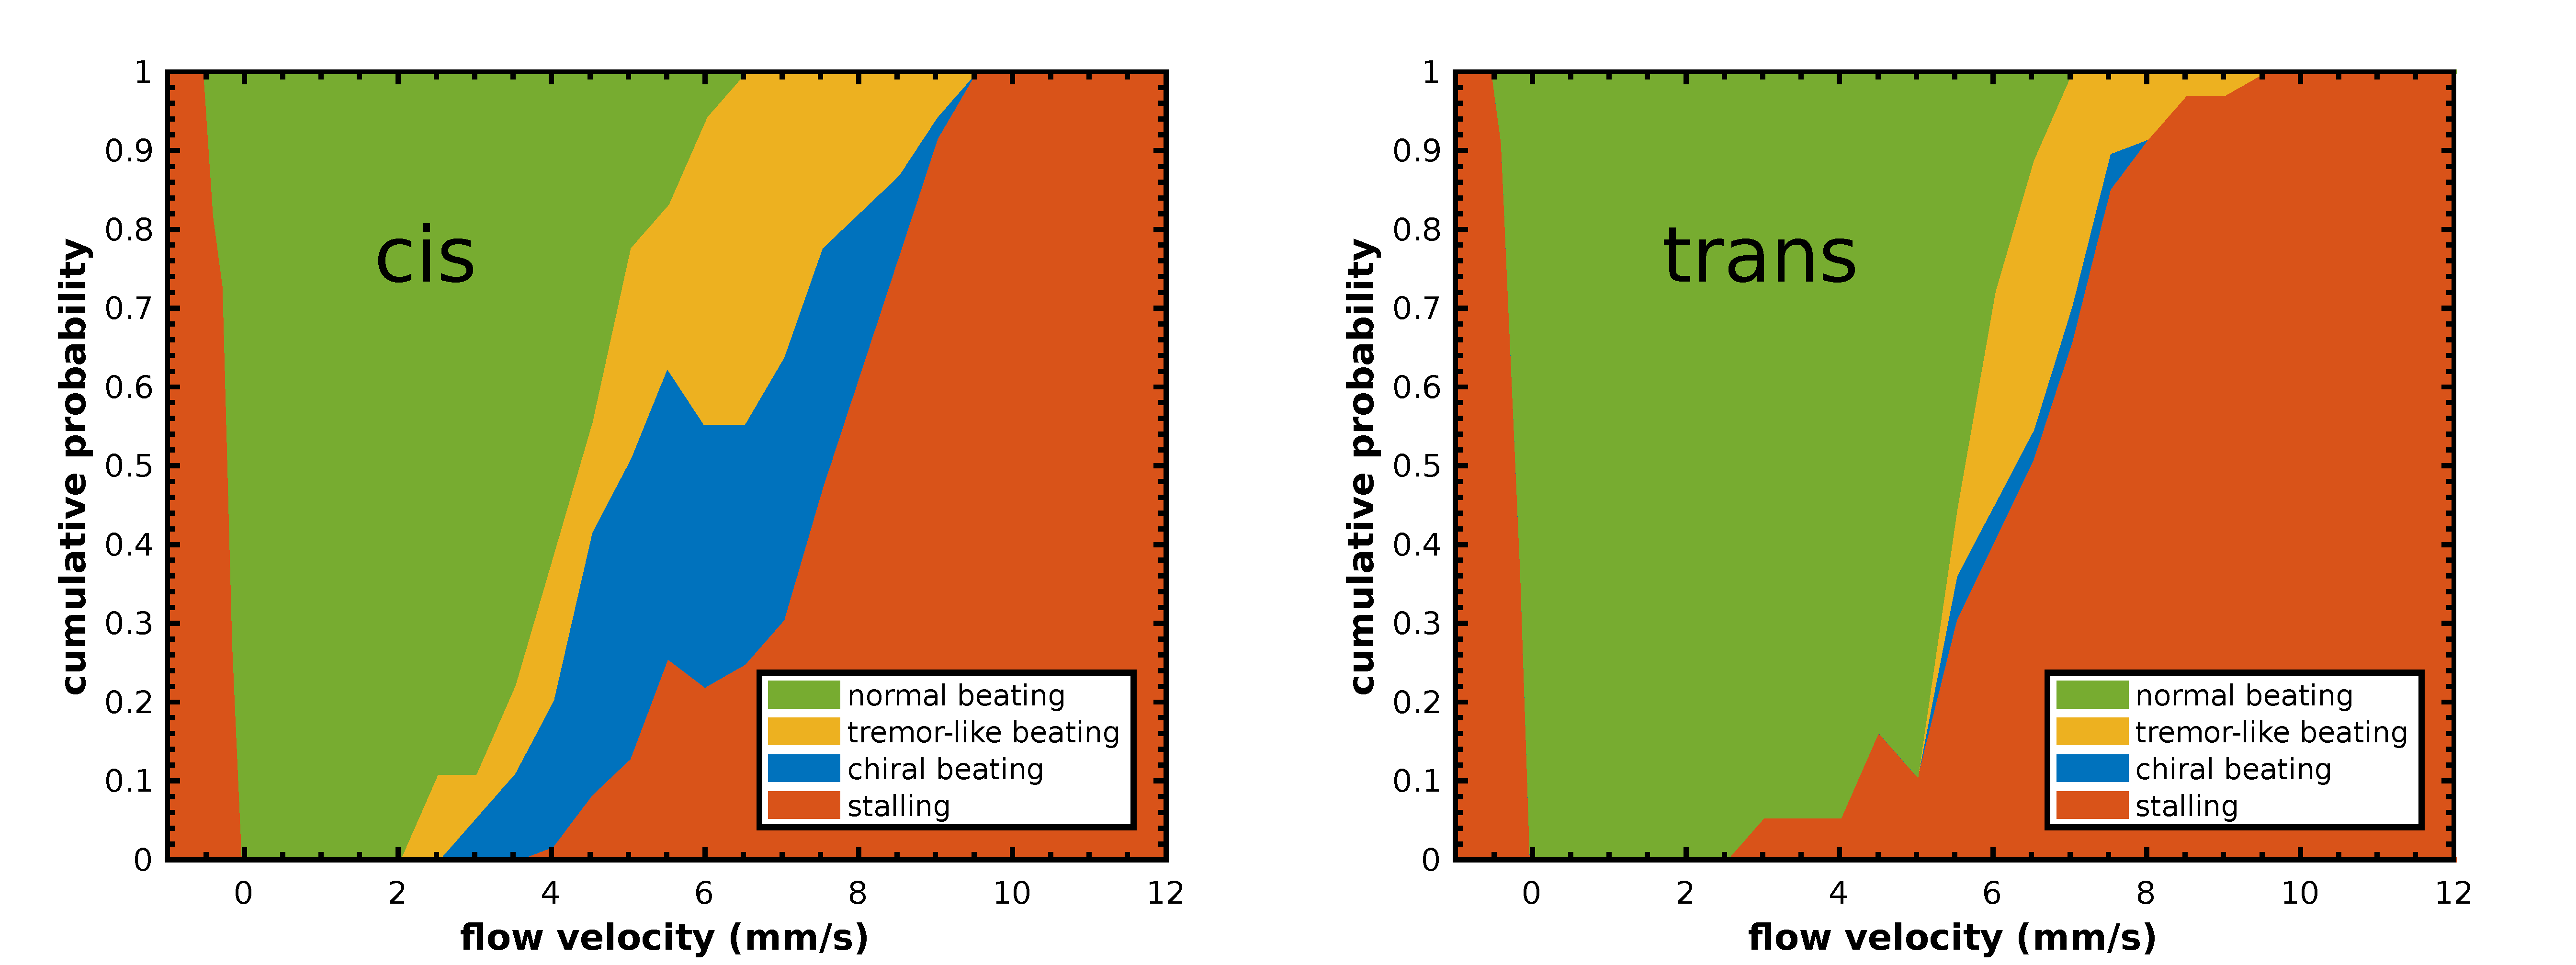
\includegraphics[width=\textwidth,keepaspectratio]{stalling_statistics.pdf}}{}\vskip2ex
                \small{
                    \begin{itemize}
                        \item \textcontour{black}{chiral beating is almost exclusive to the cis flagellum}
                        \item \textcontour{black}{tremor-like beating is less pronounced for the trans flagellum}
                        \item \textcontour{black}{trans flagellum stalls at lower flow speeds than cis flagellum}
                    \end{itemize}
                }
            \end{center}
            \vfill
        \end{frame}


\section{}
    \subsection{}
        \begin{frame}
%             \frametitle{\Large{Summary}}
            \begin{center}
                \textcontour{black}{\large\textbf{Technical summary}}\hfill
                \small{
                    \begin{itemize}
                        \item \textcontour{black}{optical tweezers are versatile but lack trapping power and orientational control}
                        \item \textcontour{black}{micropipettes are not contactless but guarantee strong and stable orientational fixation}
                        \item \textcontour{black}{device control toolboxes enable fast prototyping \& reliable, fully automated measurements}
                        \item \textcontour{black}{high precision flagellar tracking permits new insights into the dynamics of flagellar beating}
                    \end{itemize}
                }\vspace{4em}
                \textcontour{black}{\large\textbf{Scientific summary}}\hfill
                \small{
                    \begin{itemize}
                        \item \textcontour{black}{flagellar load response is phase-dependent}
                        \item \textcontour{black}{load response is different for cis and trans}
                        \item \textcontour{black}{different dynamic modes of beating}
                        \item \textcontour{black}{pronounced stalling hysteresis under positive load}
                        \item \textcontour{black}{no stalling hysteresis under negative load}
                        \item \textcontour{black}{flagella can sustain very high positive load but only small negative load}
                    \end{itemize}
                }
            \end{center}
            \vfill
        \end{frame}


\appendix
    \begin{frame}
        \begin{center}
            \Large\textcontour{black}{\textbf{Thank you for your attention!}}
        \end{center}
    \end{frame}

\end{document}
